\chapter[Eletrônica]{Eletrônica}

\section{Implementação}
A partir dos requisitos de projeto e das soluções propostas no ponto de controle 01, foi implementado os seguintes subsistemas. 
\begin{itemize}
\item Controle de temperatura
\item Controle de saída chopp
\item Atuação de motores
\item Abertura do reservatório de copos

\end{itemize}
  
  Os códigos utilizados neste trabalho encontram-se em controle de versão na ferramenta GitHub e podem ser facilmente acessados em: \url{https://github.com/autochopp/embedded_electronics}. 

\subsection{Controle de temperatura}
	Para realizar o controle da temperatura, permitindo que o chopp esteja sempre gelado quando da retirada, foi utilizado o sensor de temperatura DS18B20 presente na Figura \ref{sensor-temperatura} , este sensor permite a leitura de temperatura até mesmo em ambientes úmidos, tal qual esta aplicação. O sensor descrito mede temperaturas entre   $ -55 ^\circ C$ e $125 ^\circ C$ com erro de $\pm 0.5 ^\circ C$. O sensor convencionado de ser posicionado na saída de chopp permitindo uma leitura mais fidedigna da temperatura real do chopp, pois na saída o chopp já circulou por toda a serpentina e estará mais próximo do equilíbrio térmico. O modo como esse sensor é conectado pode ser visto na Figura \ref{esquema-temperatura}.

\begin{figure}[!htb]
            \centering
         	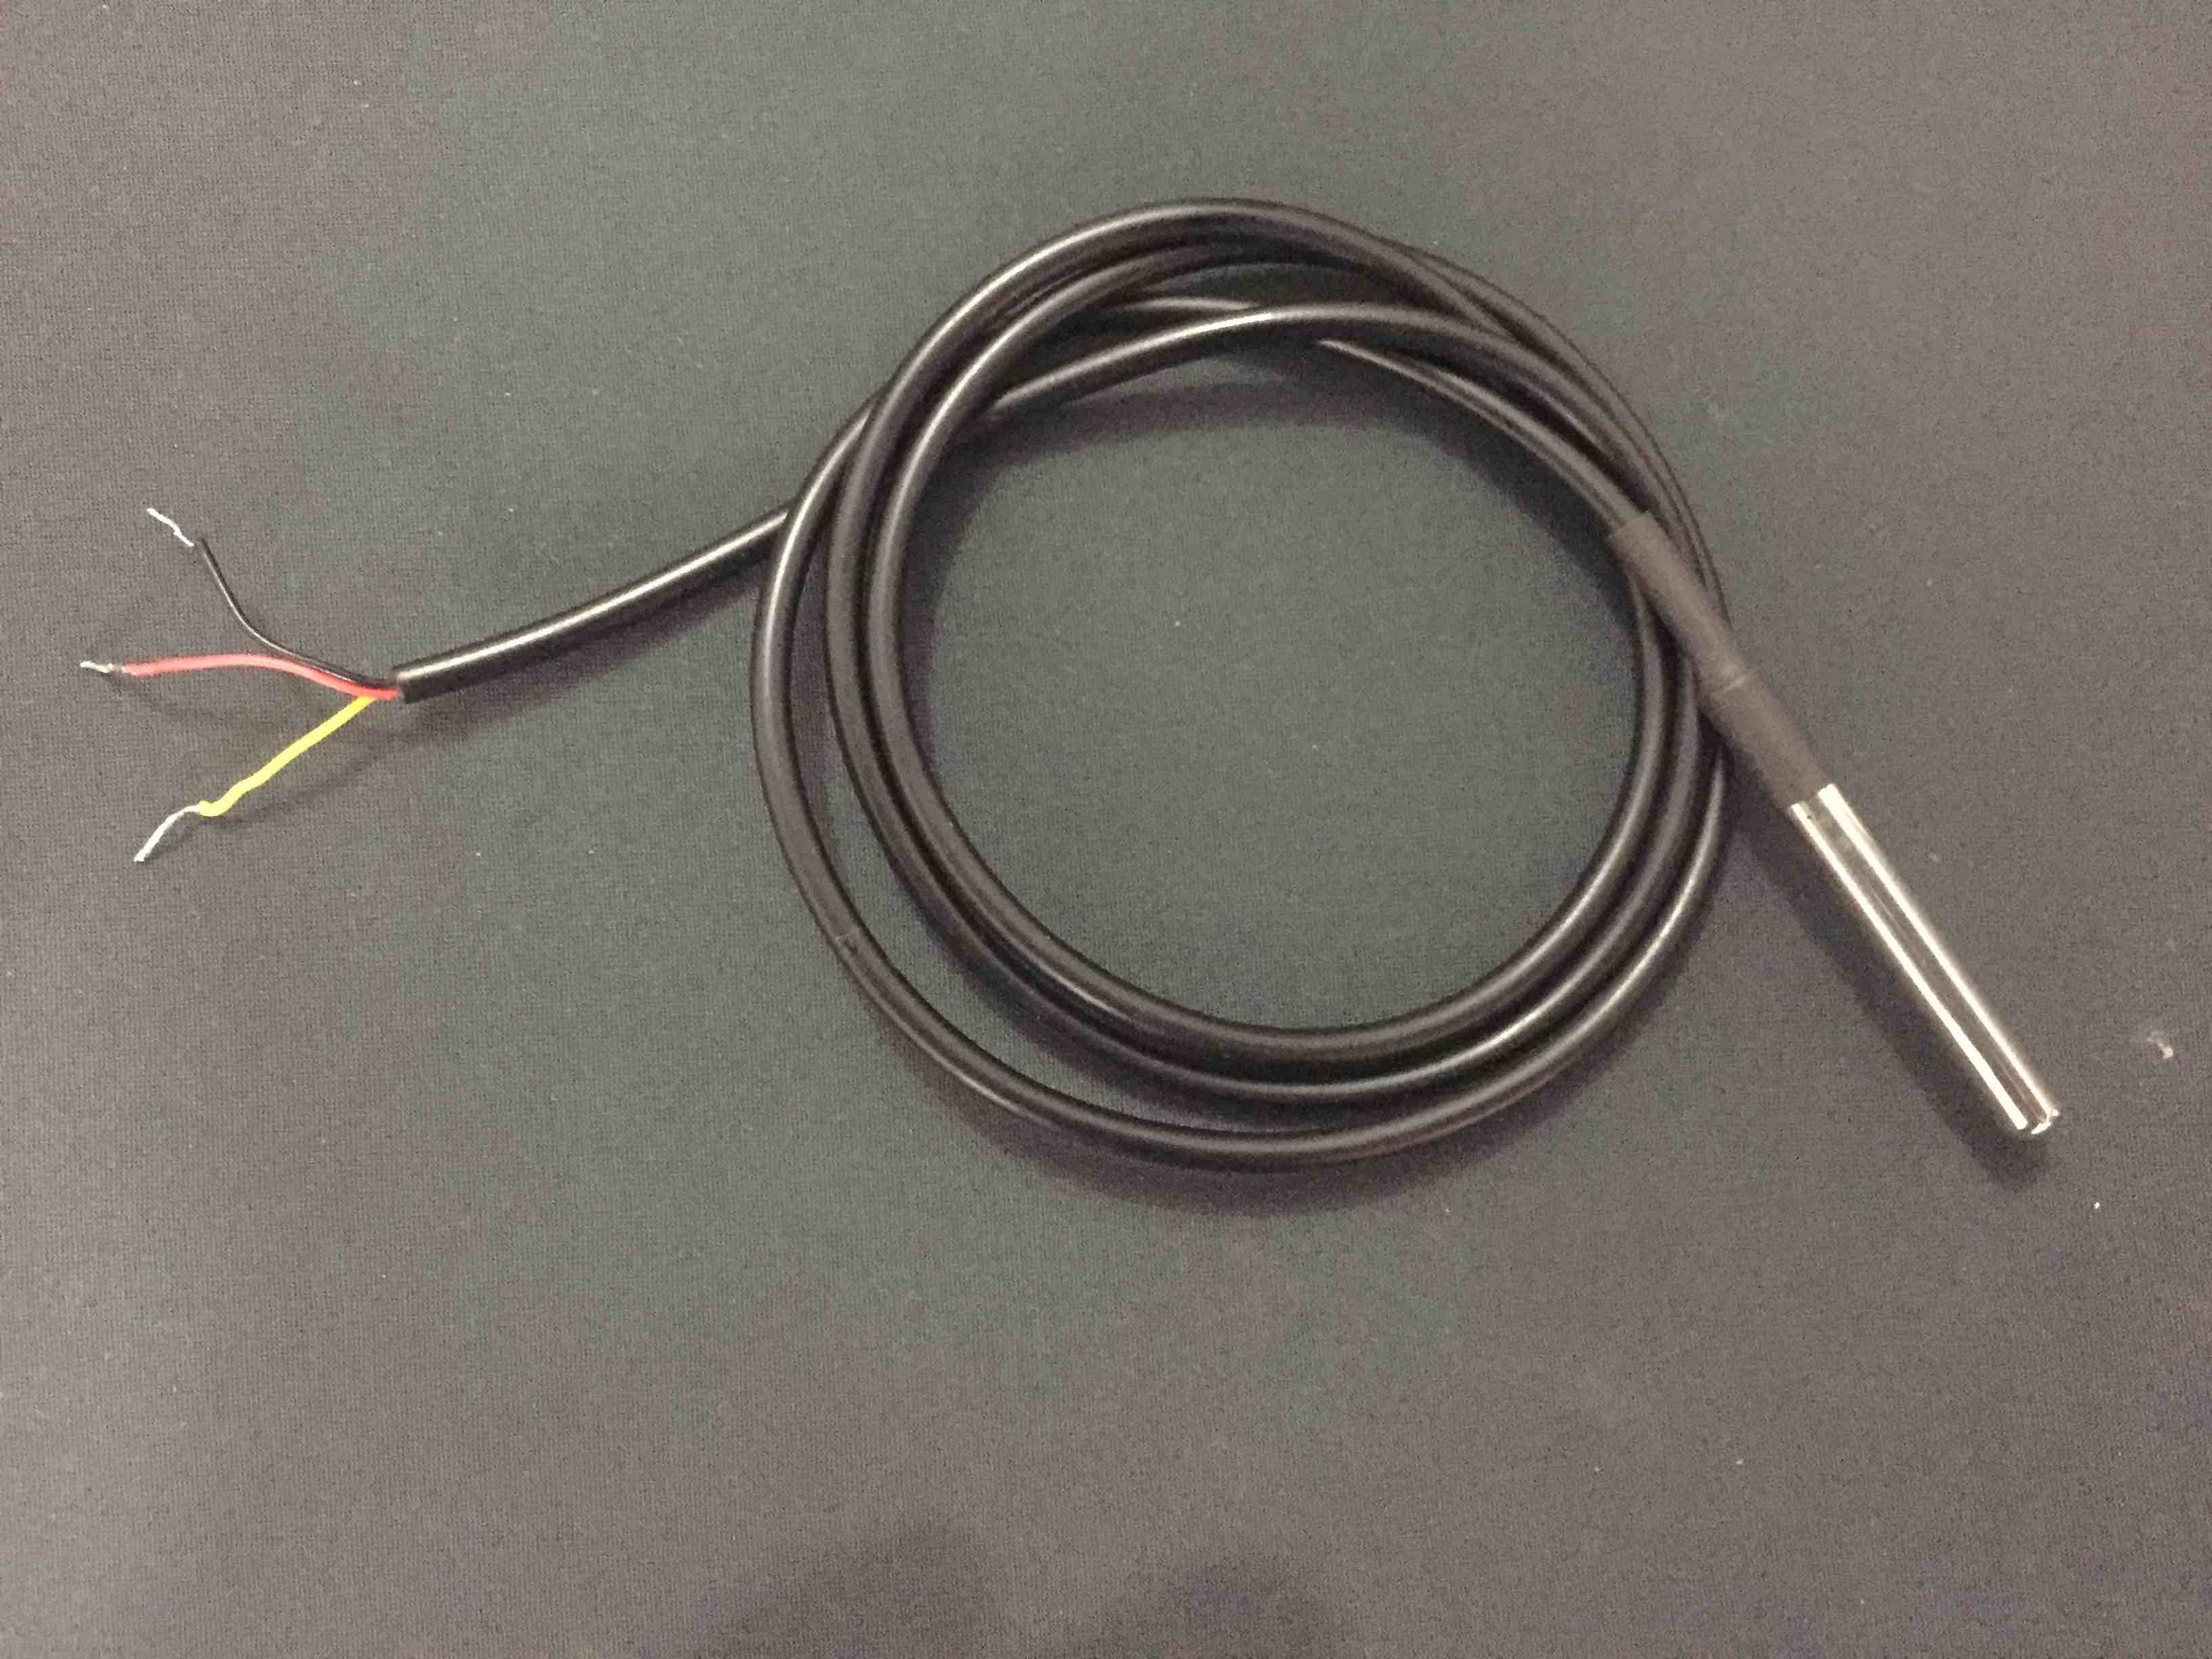
\includegraphics[scale= 0.1]{figuras/temperatura.jpg}
            \caption{Sensor de temperatura DS18B20. Fonte: Própria.}
            \label{sensor-temperatura}
\end{figure}
               
	A medição da temperatura irá permitir a ativação do compressor mantendo a temperatura na faixa ideal entre $-1$ e $1 ^\circ C$. Tal ativação será realizada pelo acionamento de um módulo relé  ligado ao compressor. 
    
\begin{figure}[!htb]
           \centering
           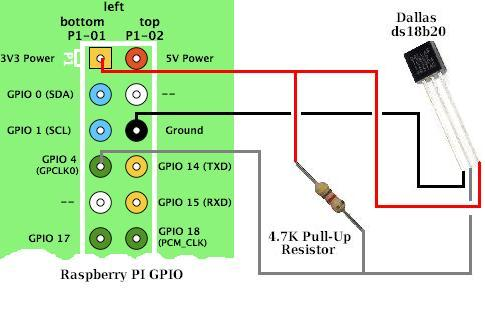
\includegraphics[scale= 0.8]{figuras/esquema.jpg}
            \caption{Esquemático do sensor de temperatura. Imagem da internet.}
            \label{esquema-temperatura}
\end{figure}    
    
   


\subsection{Controle de saída de chopp}
\subsubsection{Presença do copo}
Antes de que se possa tirar o chopp, há a necessidade de se verificar a presença do copo no sistema. Para tanto, inicialmente utilizou-se o sensor ultrassônico HC-SR04, porém, o mesmo inviabilizou seu uso devido a complexidade de sua comunicação com o computador (\textit{Raspberry pi}).

Como solução mais direta e que evitaria tal nível de complexidade, optou-se por utilizar um sensor de trila, que se comunica de forma direta com o computador e retorna um valor binário para a presença ou não do copo. Uma consequência dessa escolha é a necessidade de uma tira preta no copo, sendo a mesma posicionada embaixo do copo, que, deste modo, não interfere com a experiência do usuário.
 		%IMAGENS 
\subsubsection{Controle de fluxo}
Para que se pudesse ter um controle do volume presente no copo e consequentemente volume restante nos reservatórios inicialmente pensou-se em utilizar dois sensores (por redundância), sendo eles o sensor de fluxo YFS201 e uma célula de carga.

Obtiveram-se resultados satisfatórios com o sensor de fluxo, porém verificou-se um erro muito grande em suas medidas, o qual chegava a dez porcento nos testes efetuados. Já quanto ao sensor de carga, não houve sucesso em sua implementação, apresentando resultados quase que aleatórios.

Após discutir o presente problema com professores e orientadores, outra solução foi proposta. A solução proposta se utiliza de diodos emissores de luz e fototransistores posicionados a uma distância conhecida. Sabendo-se a bitola do tubo utilizado e, contando-se o tempo entre os acionamentos, pode-se calcular o fluxo passante.  

\subsubsection{Controle de colarinho}

	O controle do colarinho é feito através da atuação de motores, estes que irão movimentar a alavanca que controla a saída de chopp e colarinho. Desta forma é necessário realizar medições de tempo para cada tamanho de colarinho selecionável, servindo assim a quantidade. Esse acionamento é feito por tempo e relaciona-se com a entrada de ar no  sistema.

\subsection{Atuação dos motores}
Dois dos mais importantes subsistemas que contribuem diretamente com a experiência do usuário é a inclinação do copo e tiragem automática do chopp,
para tais tarefas fez-se o uso de motores de passo.
Para o controle dos motores usou-se o microcontrolador TM4C123G embarcado na \textit{LaunchPad Tiva$^{TM}$ C Series}, o uso dessa plataforma é necessário devido ao fato de que as bobinas dos motores devem funcionar constantemente, para não interrupção do serviço,optou-se pelo o uso da mesma.


Os motores são alimentação com uma de 12V, para isso usou-se uma fonte de energia externa, devido ao consumo de corrente dos motores ser superiores ao que se pode fornecer com o microcontrolador, fez-se necessário o uso de um \textit{driver} L298N. A Figura \ref{motor} mostra o sistema dos motores montado.

\begin{figure}[!h]
            \centering
         	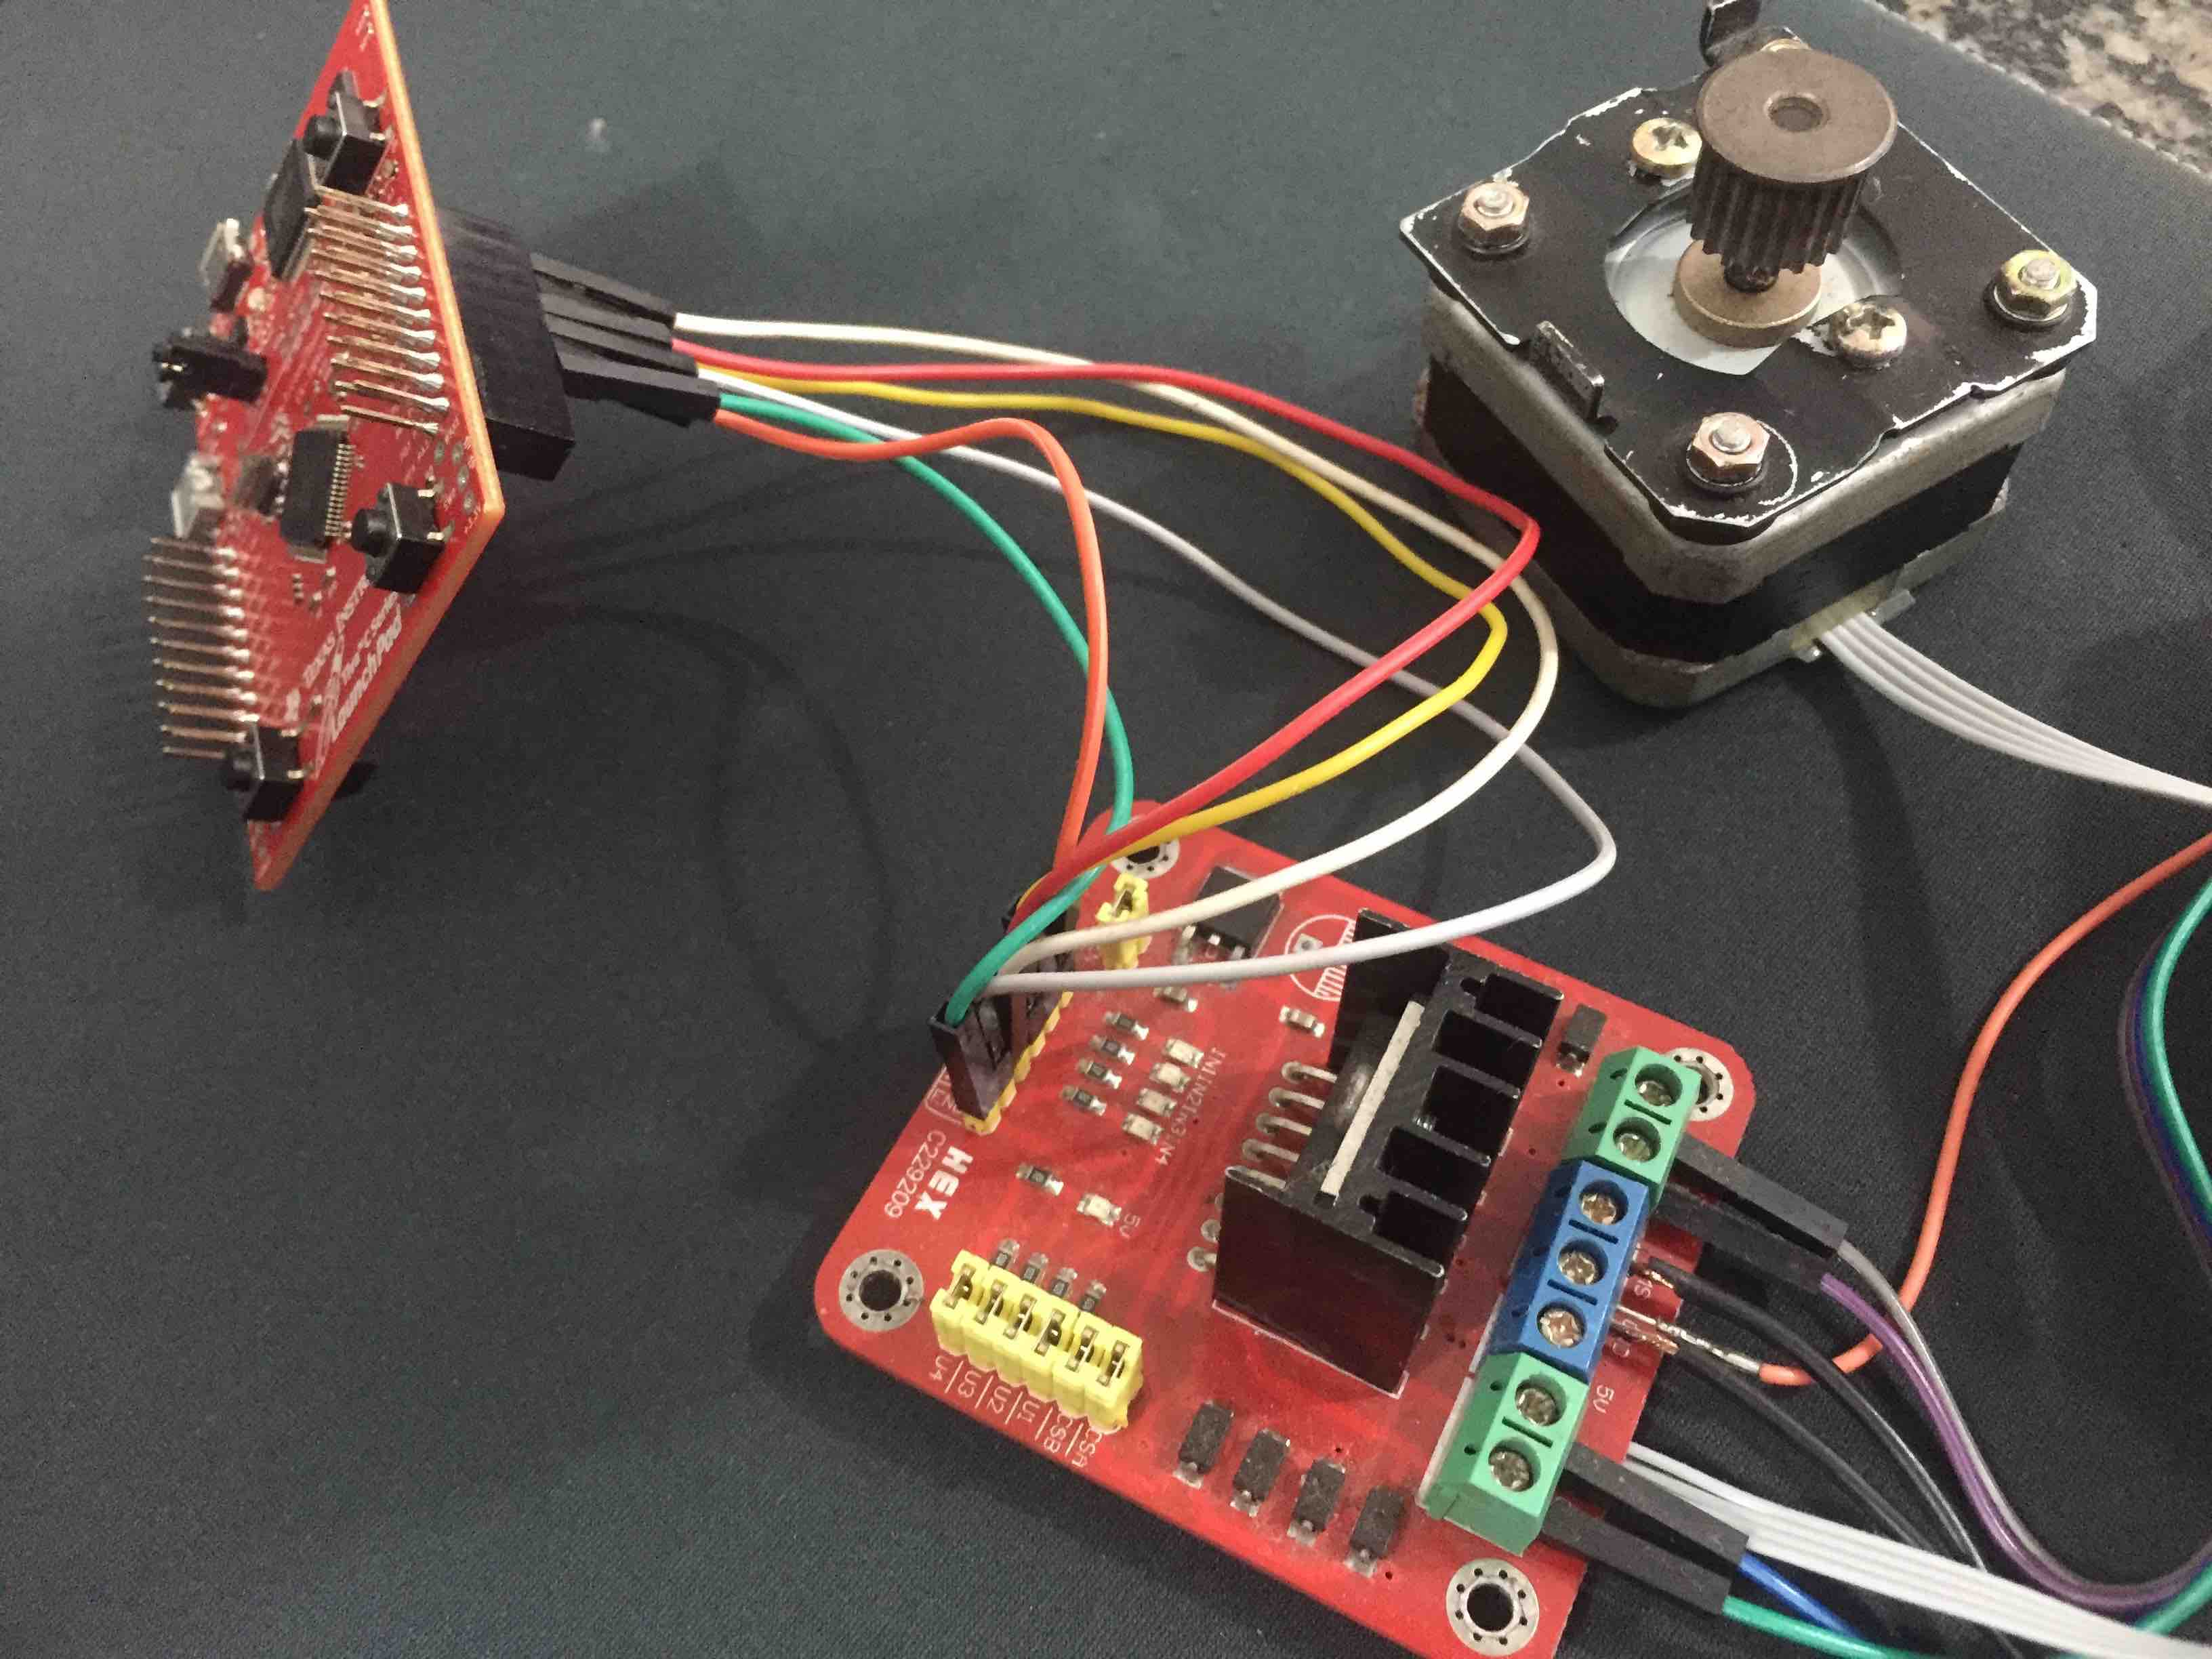
\includegraphics[scale= 0.1]{figuras/motor.jpg}
            \caption{Sistema de acionamento de motor de passo.}
            \label{motor}
\end{figure}

\newpage
\subsection{Abertura do reservatório de copos}

 Esse serviço se fez necessário, após a decisão de disponibilizar o copo ao usuário, portanto os copos devem ser armazenados na própria máquina. Para disponibilizar os copos, eles estarão dispostos de forma que sempre que exista uma requisição de um chopp, um copo caia em um reservatório próprio. Para empurrar os copos são utilizados duas solenoides de modelo TAU-0530, que pode ser visto na Figura \ref{solenoide}. 

\begin{figure}[!h]
            \centering
         	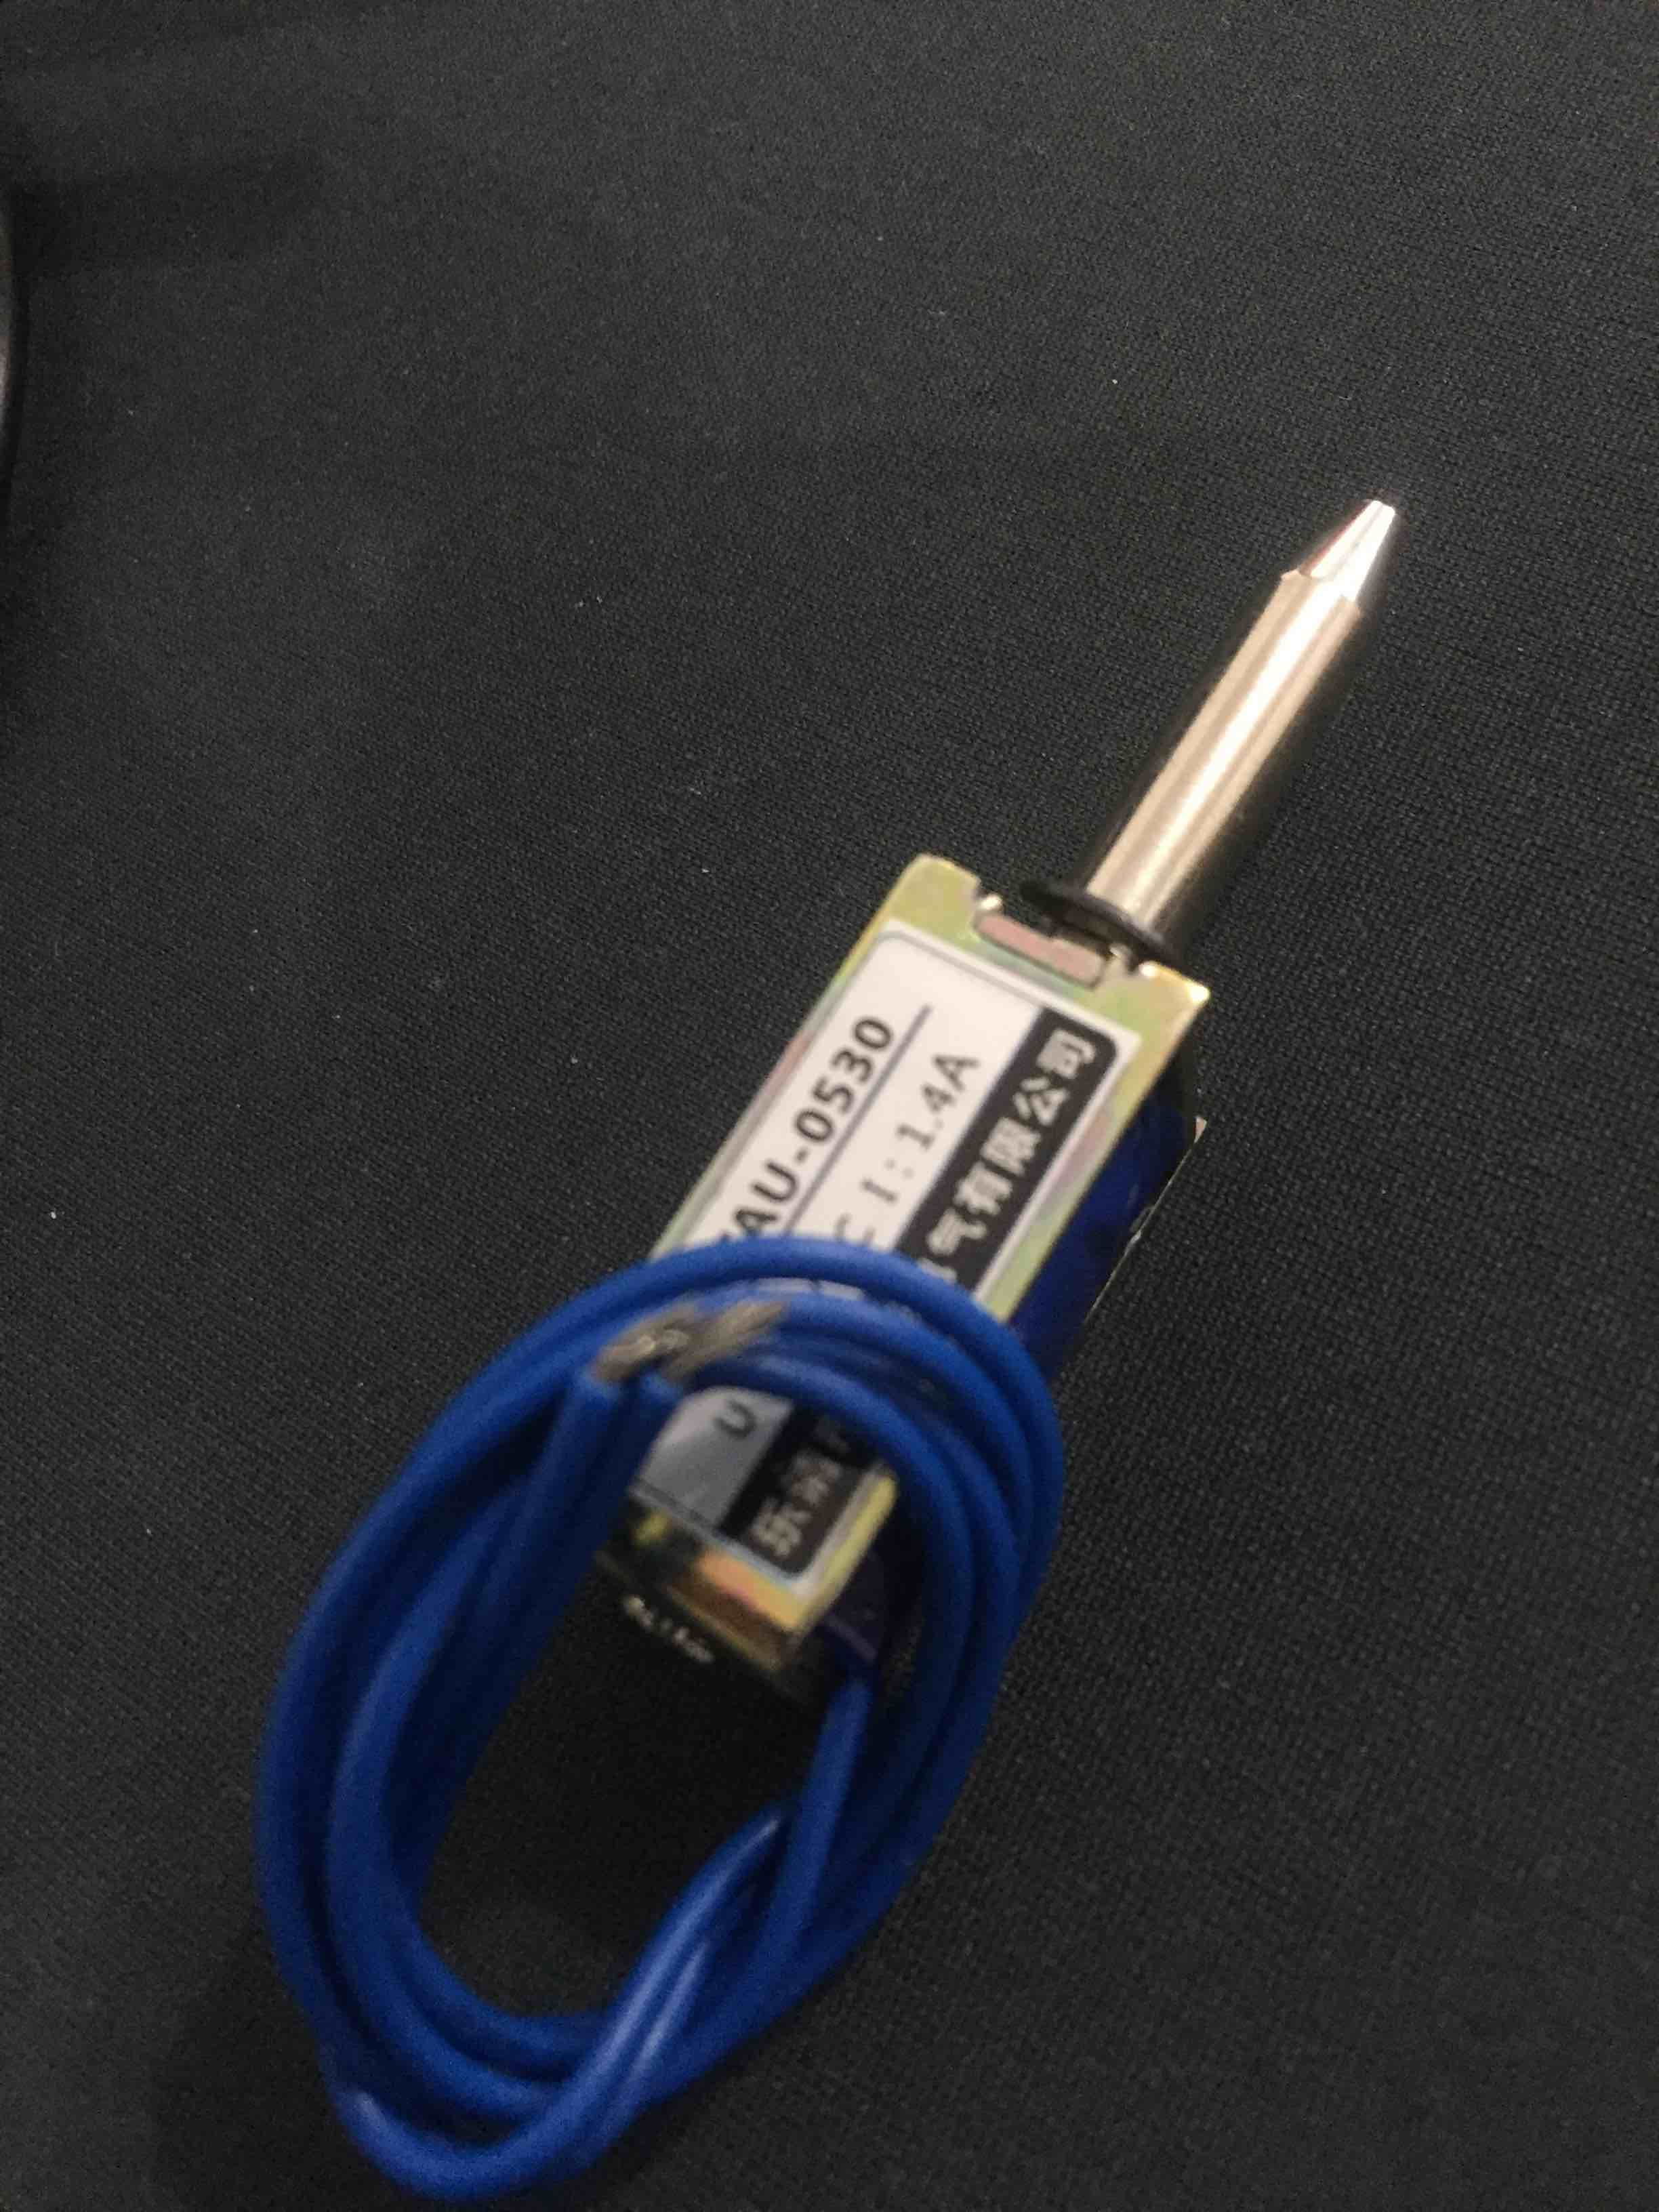
\includegraphics[scale= 0.06]{figuras/solenoide.jpg}
            \caption{Solenoide utilizado.}
            \label{solenoide}
\end{figure}

	

